\chapter{Bowling}

In this project you will create a favorite game of children - bowling. The player will have to shoot a ball from the bottom of the screen that will reach the pins located at the top. The goal is for the player to knock down all the pins.

\begin{figure}[H]
   \centering
   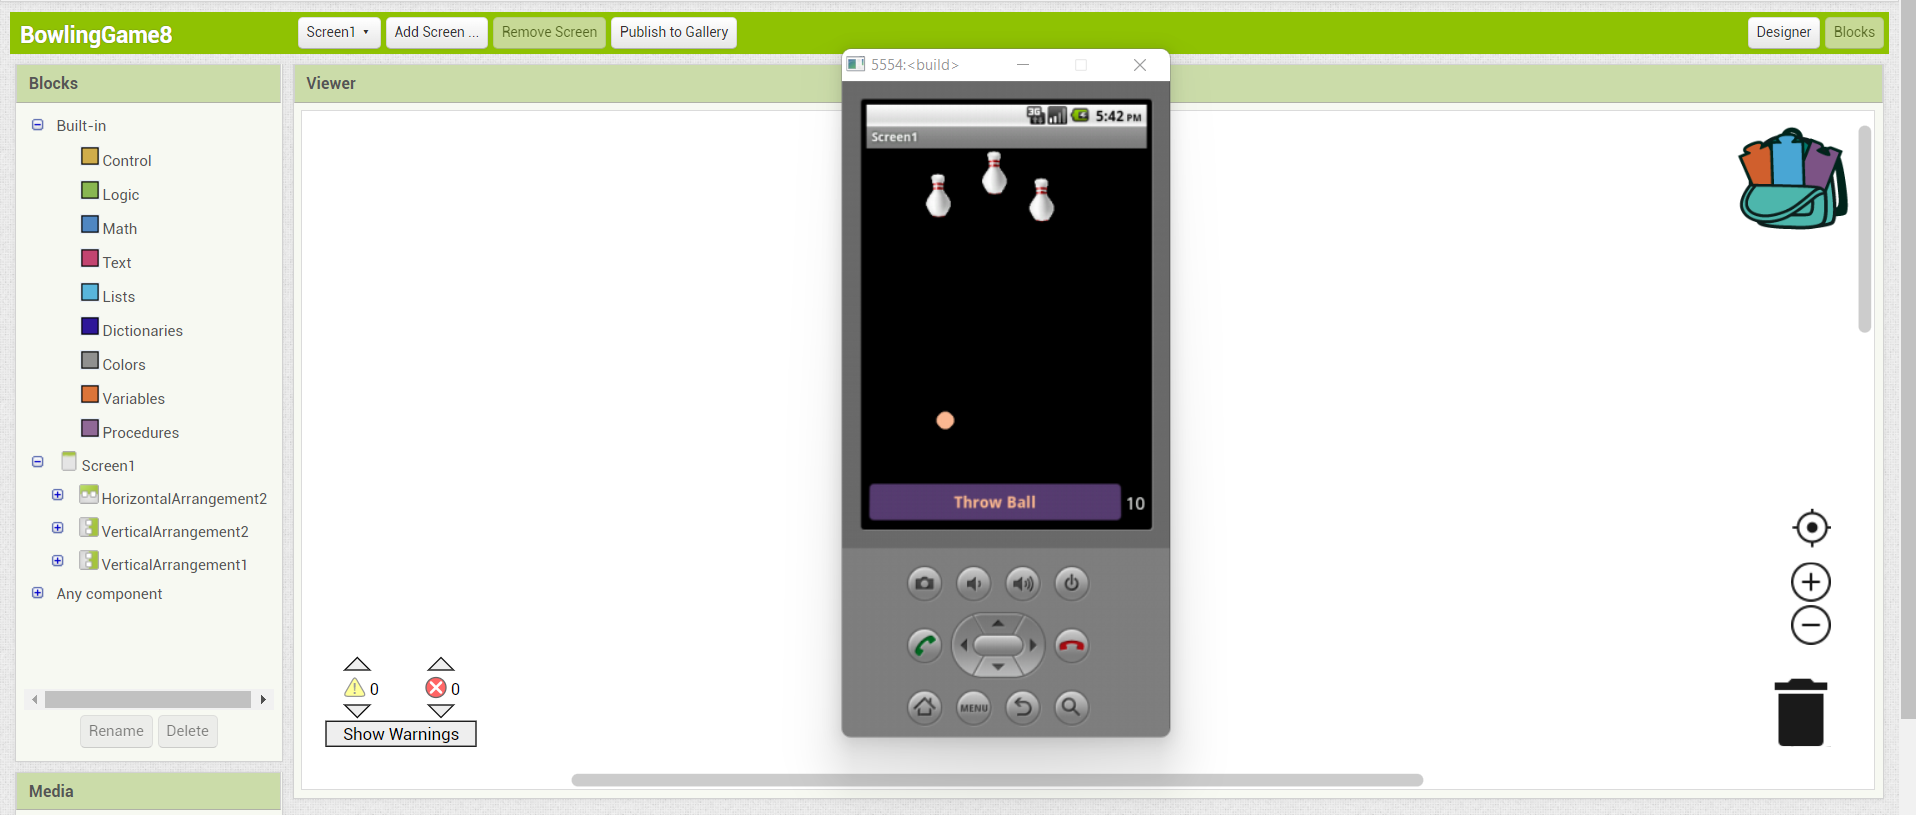
\includegraphics[width=1.0\linewidth,height=0.5\linewidth]{fig130001.png}
   \caption{Bowling}
\label{fig130001}
\end{figure}

\section{Creating the Design}

In the first step, you will create the game's home screen. There will be a button on it, which will be the start of the game. From the Layout group, the VerticalArrangement element must be added. The dimensions of the element must be the same as the dimensions of the screen. For this the height and width properties need to be changed. For the background of the game, in addition to the ready-made colors, you can also create your own color.

\begin{figure}[H]
   \centering
   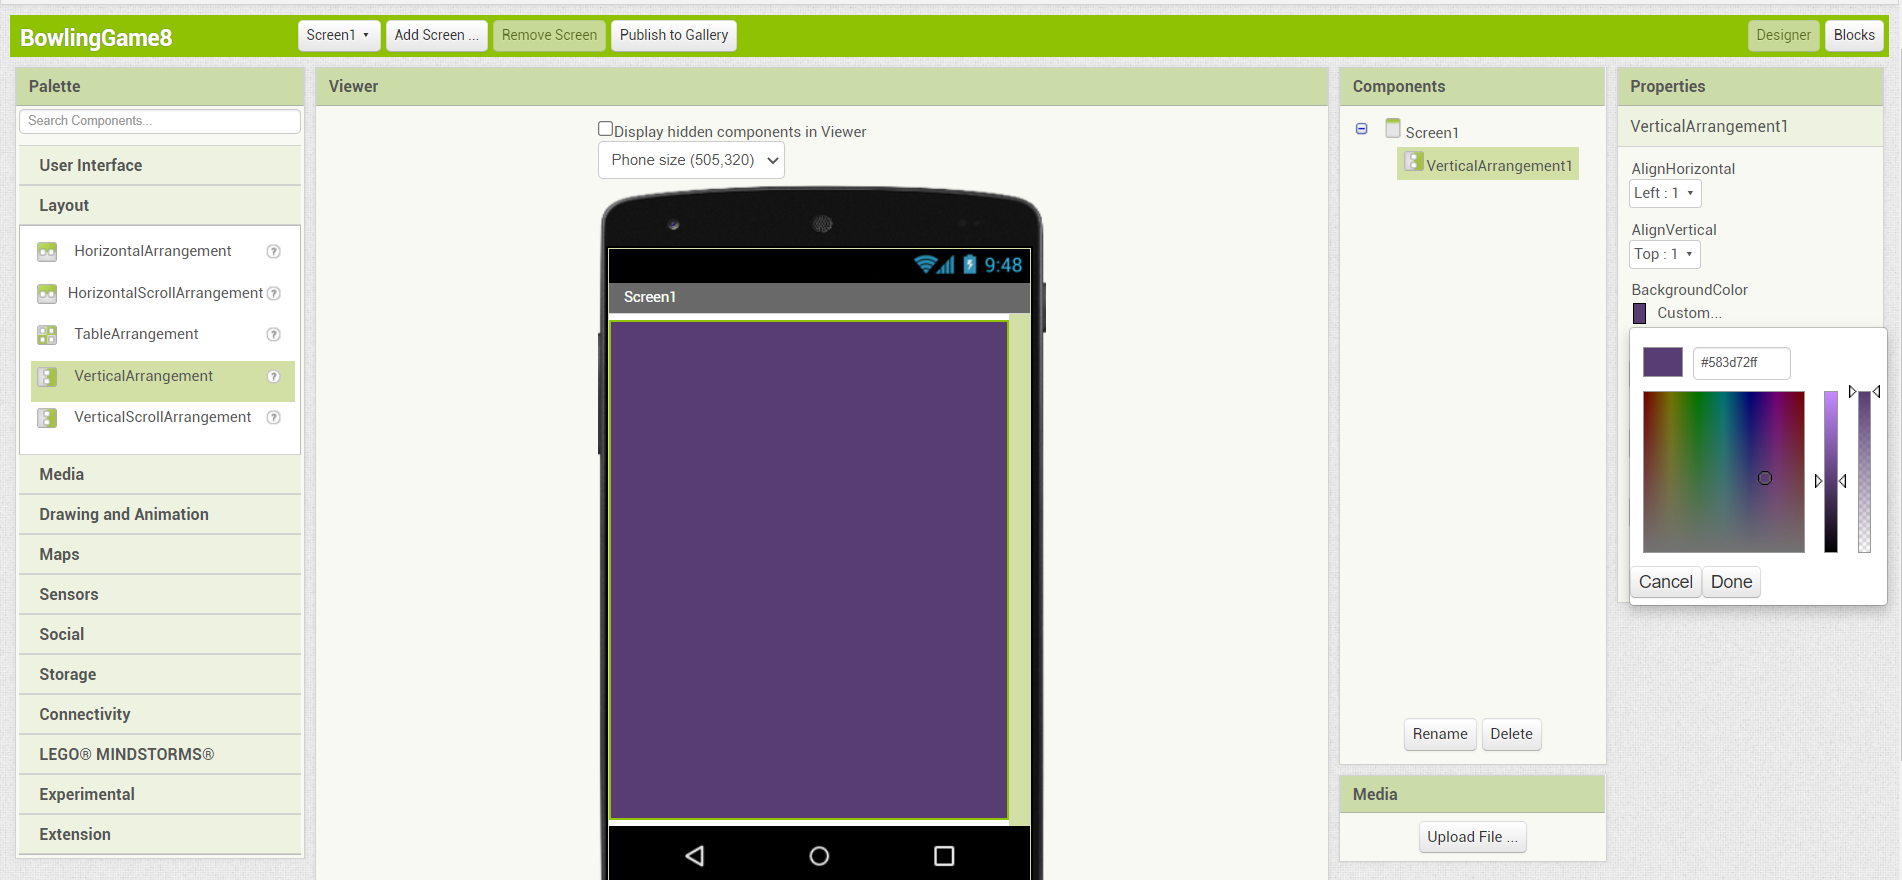
\includegraphics[width=1.0\linewidth,height=0.5\linewidth]{fig130002.png}
   \caption{Home screen}
\label{fig130002}
\end{figure}

You should also add a button to start the game. Change the design of the button and position it in the middle of the screen.

\begin{figure}[H]
   \centering
   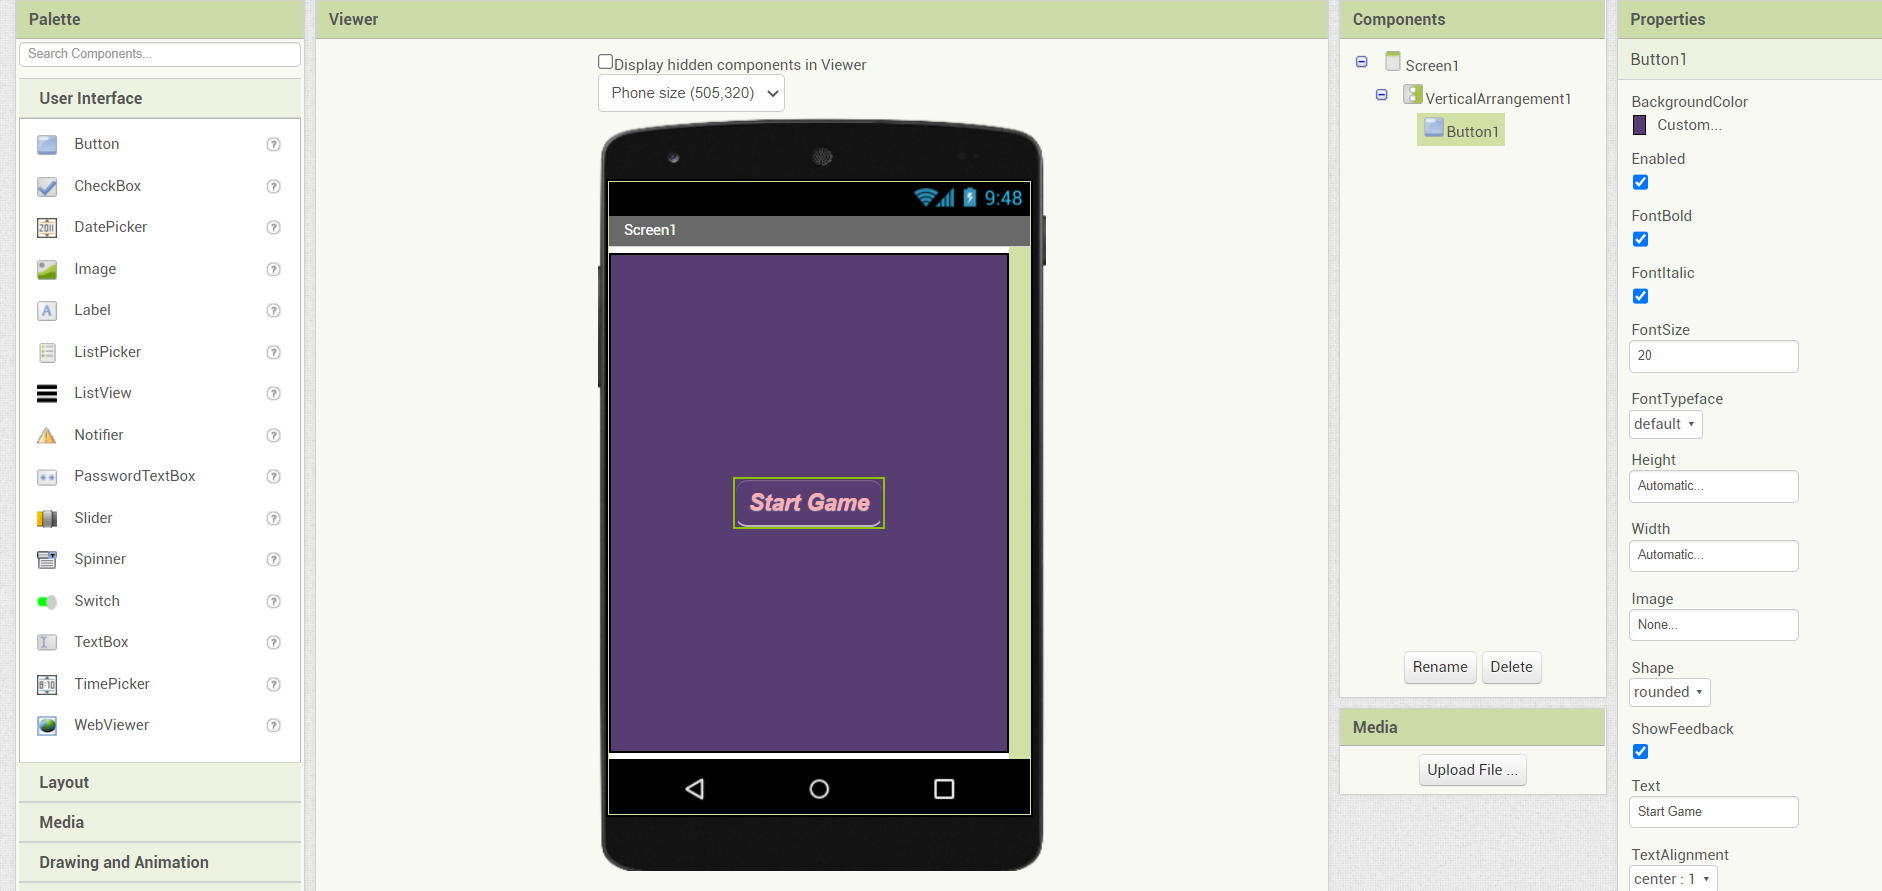
\includegraphics[width=1.0\linewidth,height=0.5\linewidth]{fig130003.png}
   \caption{Start Game Button}
\label{fig130003}
\end{figure}

In the next step, you will create the endgame screen. There will be a button on it to restart the game. You will also need to add a caption that says the game is over. First, from Layout, add a VerticalArrangment element. The dimensions of the element should again be as they are on the screen. Also choose a suitable background color for this screen.

\begin{figure}[H]
   \centering
   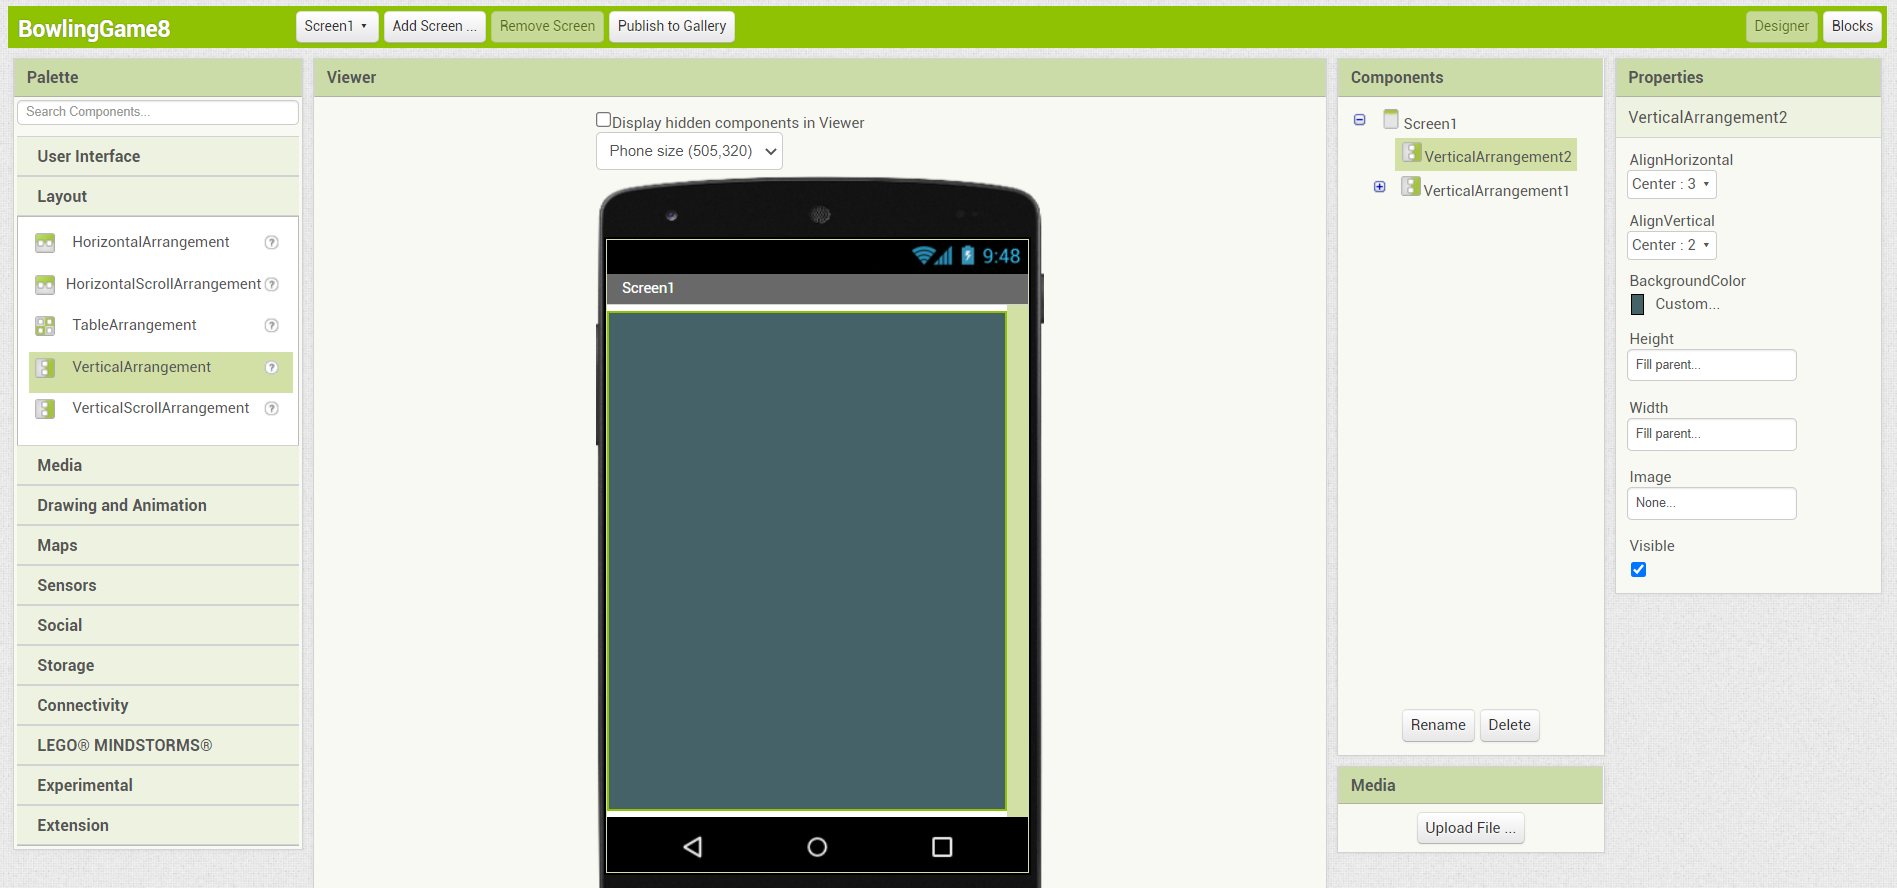
\includegraphics[width=1.0\linewidth,height=0.5\linewidth]{fig130004.png}
   \caption{End screen}
\label{fig130004}
\end{figure}

Add the button to start the game again. Change its design and position it in the middle of the screen.

\begin{figure}[H]
   \centering
   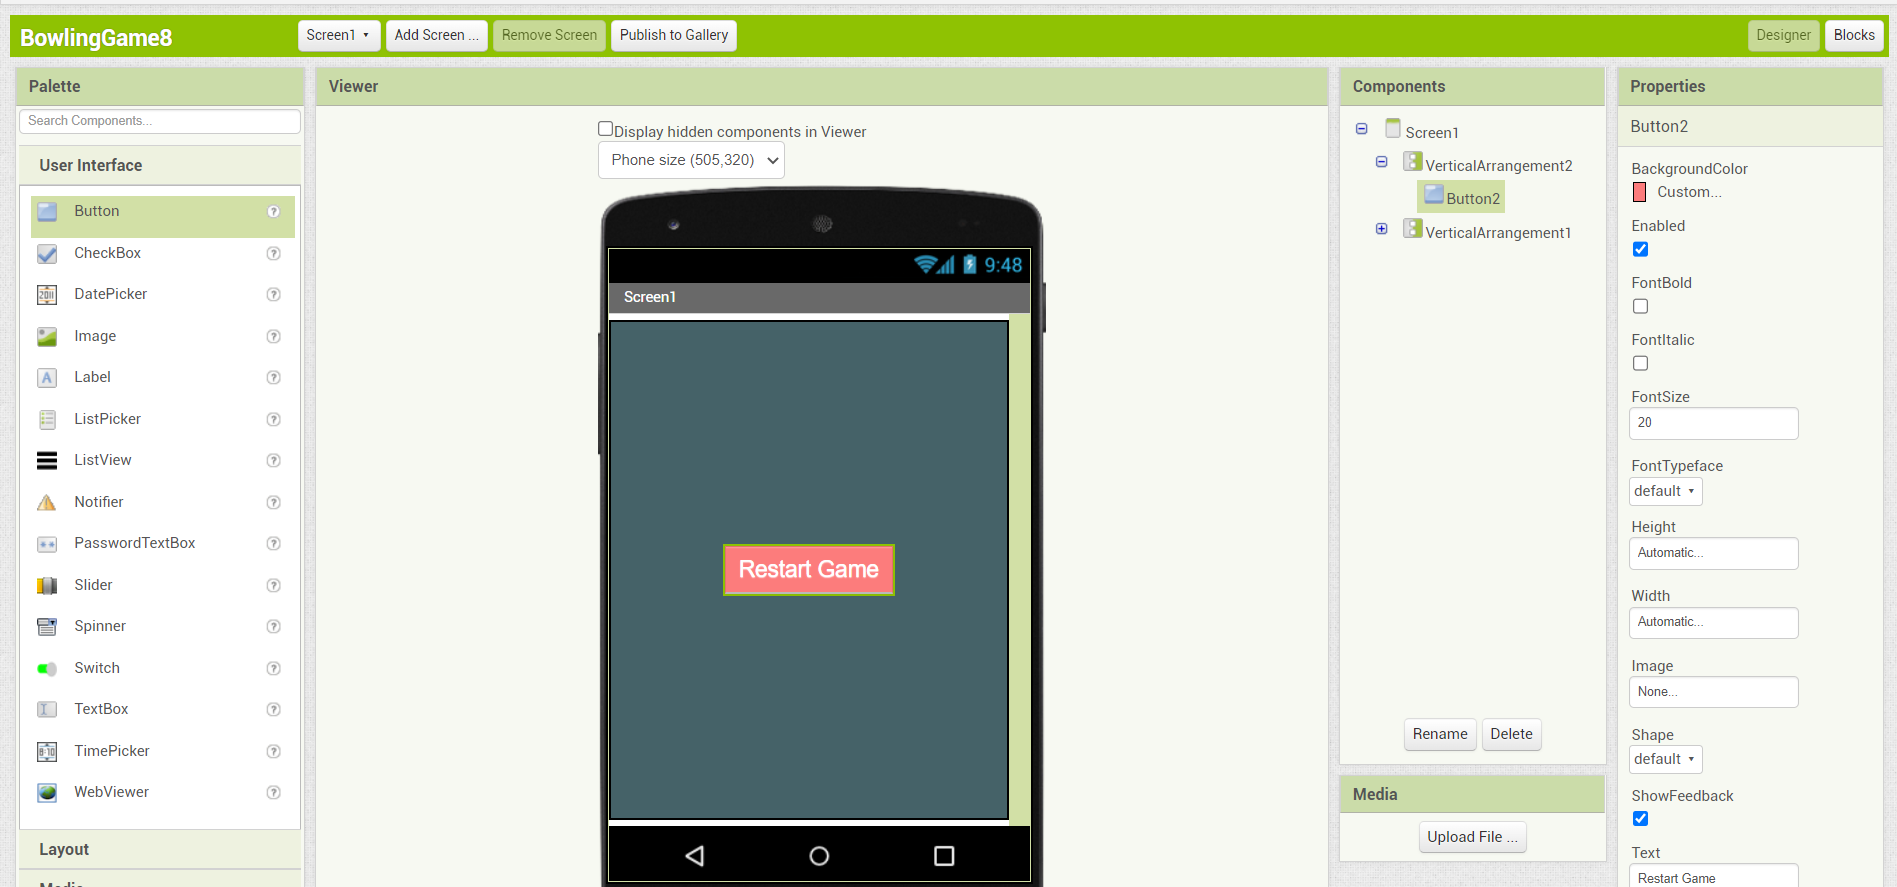
\includegraphics[width=1.0\linewidth,height=0.5\linewidth]{fig130005.png}
   \caption{Start Game Again Button}
\label{fig130005}
\end{figure}

Also add a Lable element that says Game Over.

\begin{figure}[H]
   \centering
   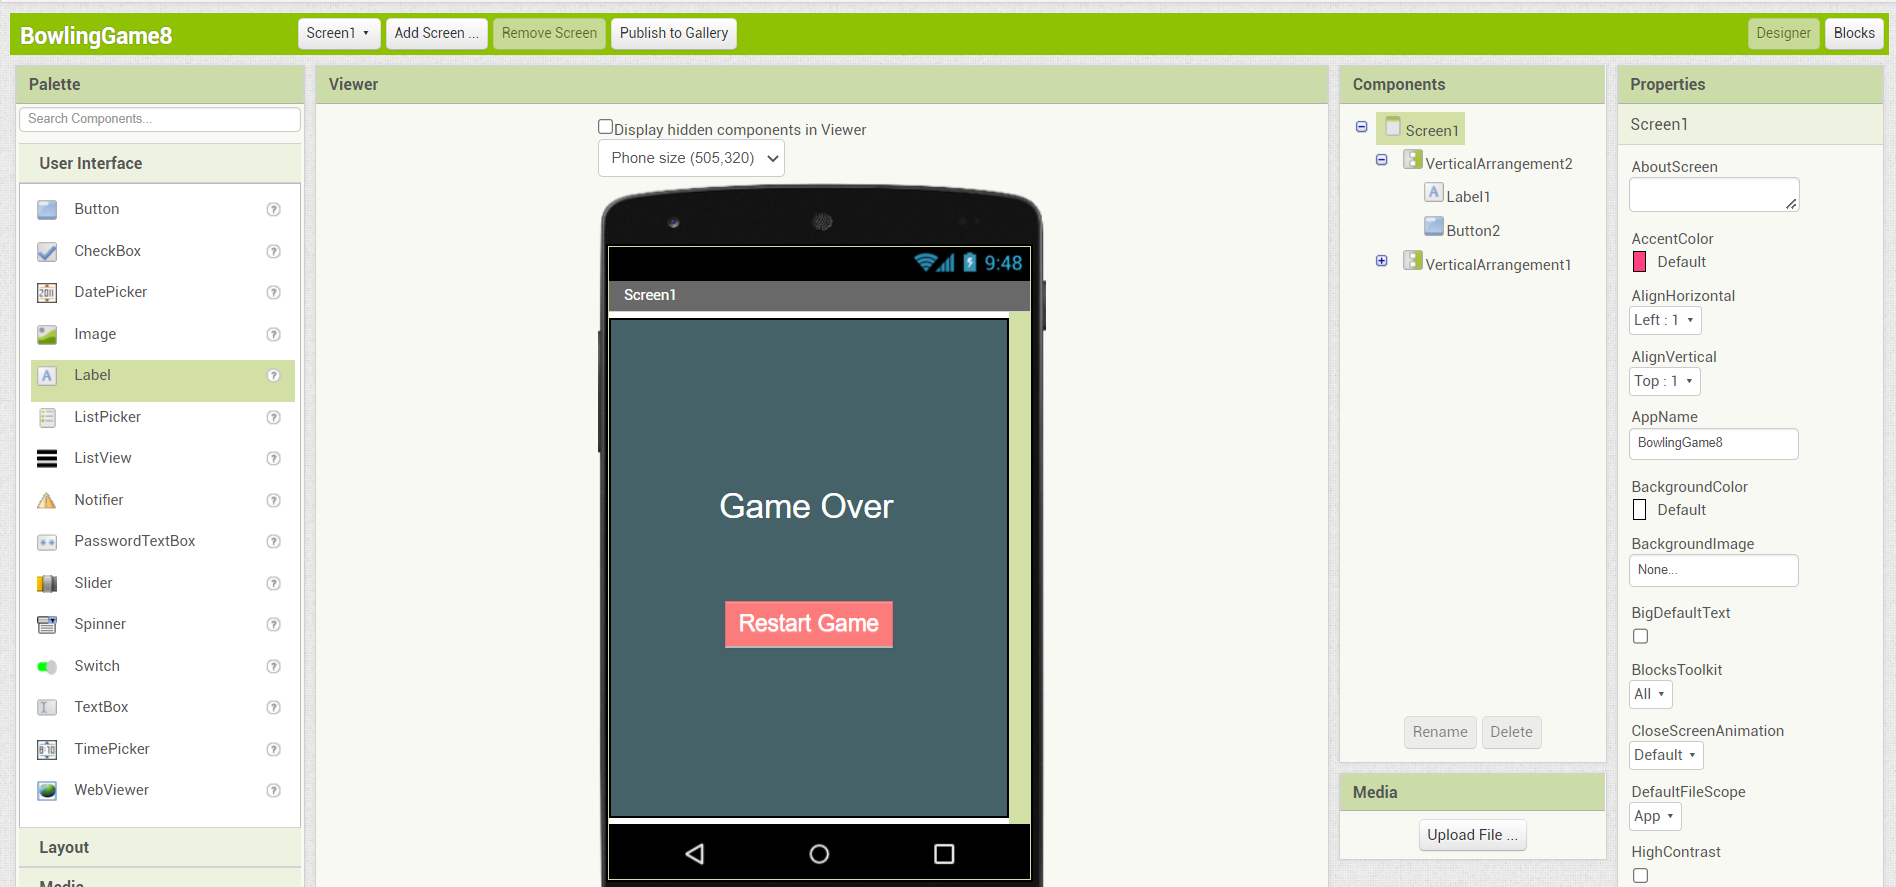
\includegraphics[width=1.0\linewidth,height=0.5\linewidth]{fig130006.png}
   \caption{End of Game Caption}
\label{fig130006}
\end{figure}

In the final step, you will create a game design. Add a VerticalArrangment element again. Resize the element so that the height and width are as they are on the screen. Inside this element, add the Canvas element from the Drawing and Animation section. Change element size and background color.

\begin{figure}[H]
   \centering
   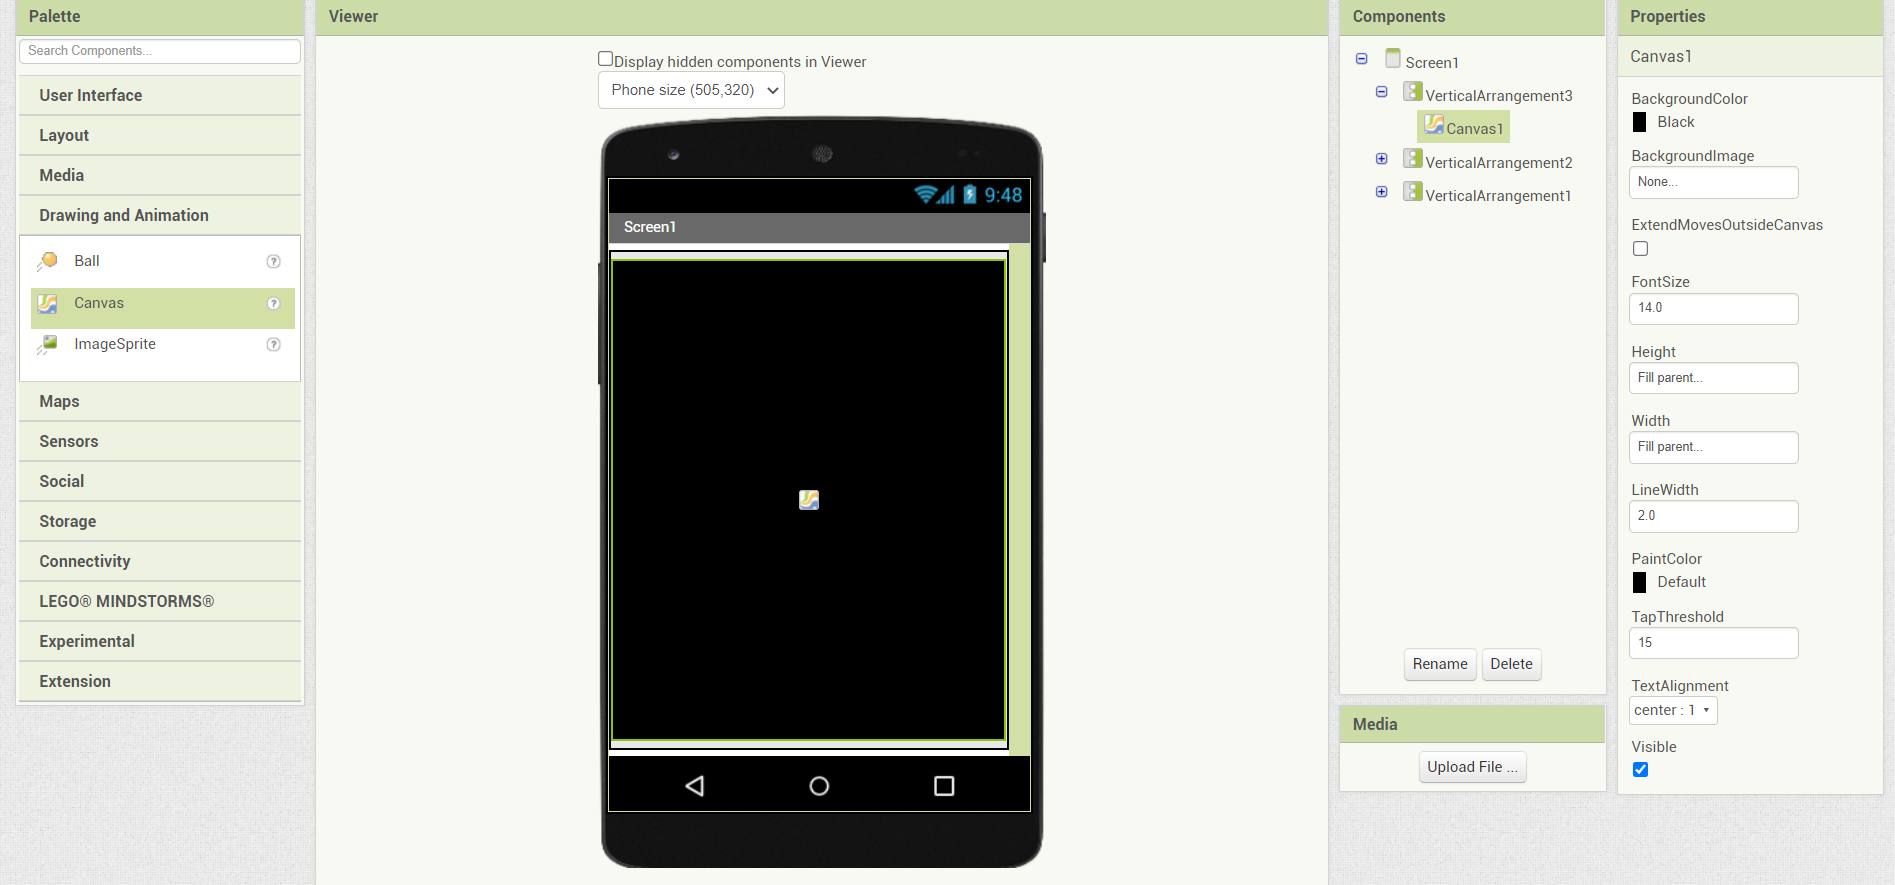
\includegraphics[width=1.0\linewidth,height=0.5\linewidth]{fig130007.png}
   \caption{Game Screen}
\label{fig130007}
\end{figure}

Add the ball element and change the dimensions, position and color of the element. The ball must be placed at the bottom of the screen.

\begin{figure}[H]
   \centering
   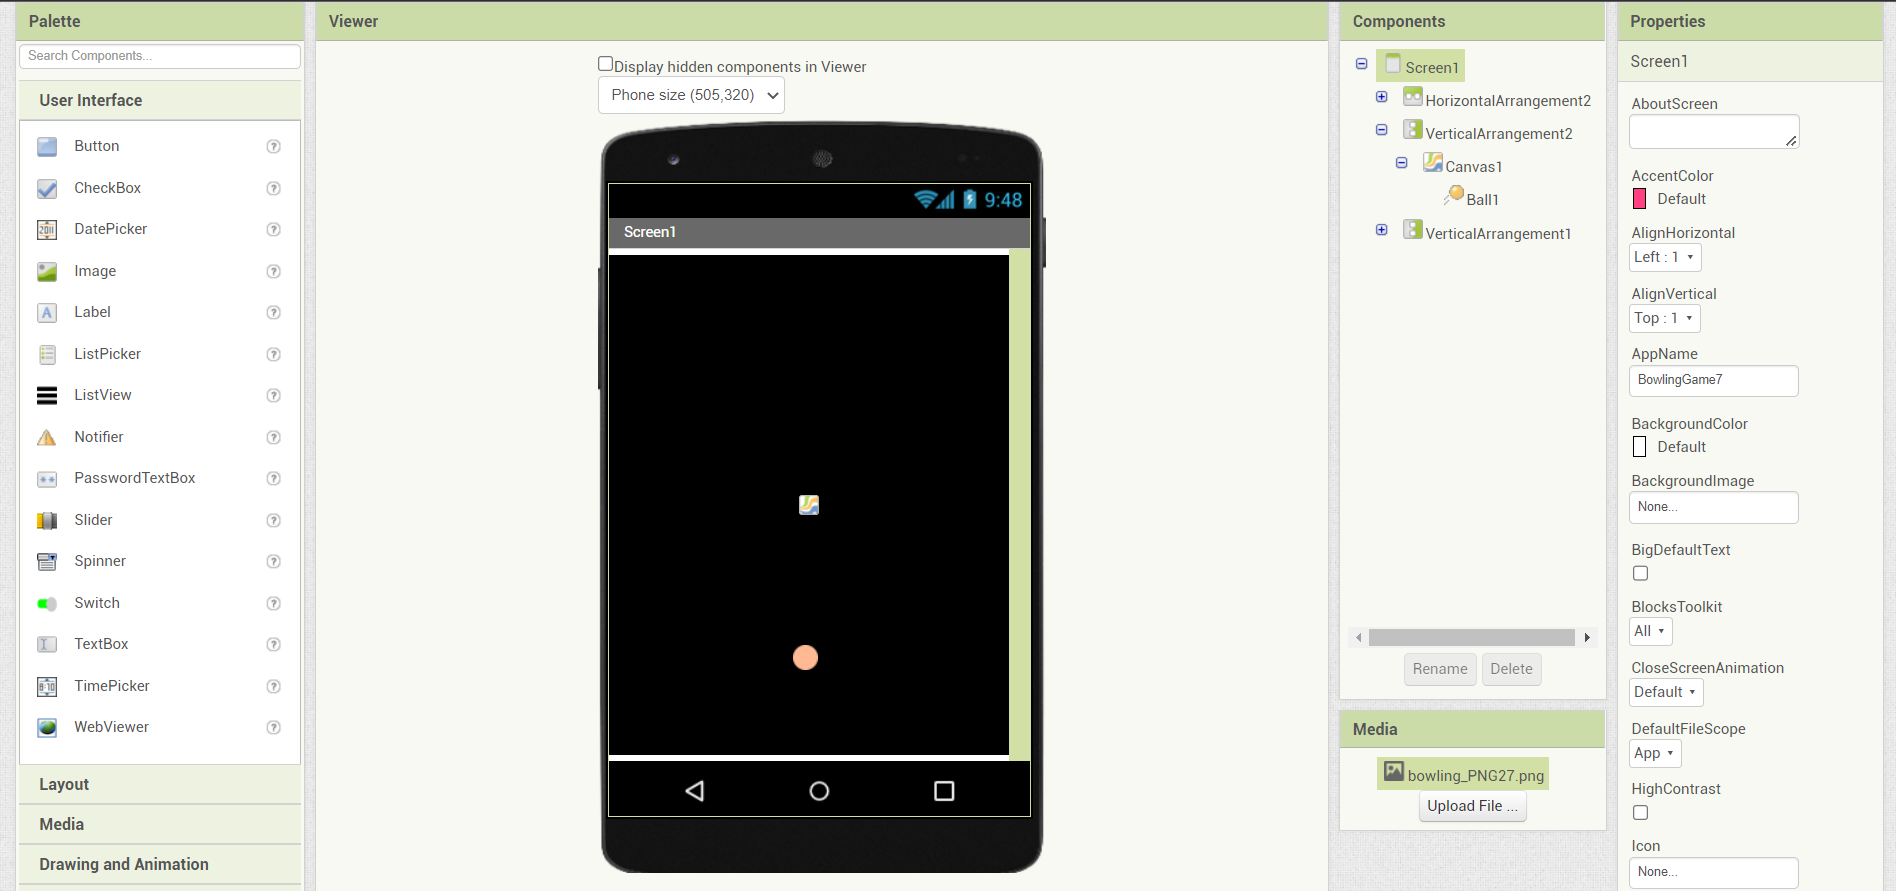
\includegraphics[width=1.0\linewidth,height=0.5\linewidth]{fig130008.png}
   \caption{Adding the ball to the game}
\label{fig130008}
\end{figure}

For the pins, you can use an image that is distributed under a free license. Add three ImageSprite elements to the Canvas element. Add the image you downloaded to each of the items. Change the dimensions and position. The three pins must be at the top of the screen.

\begin{figure}[H]
   \centering
   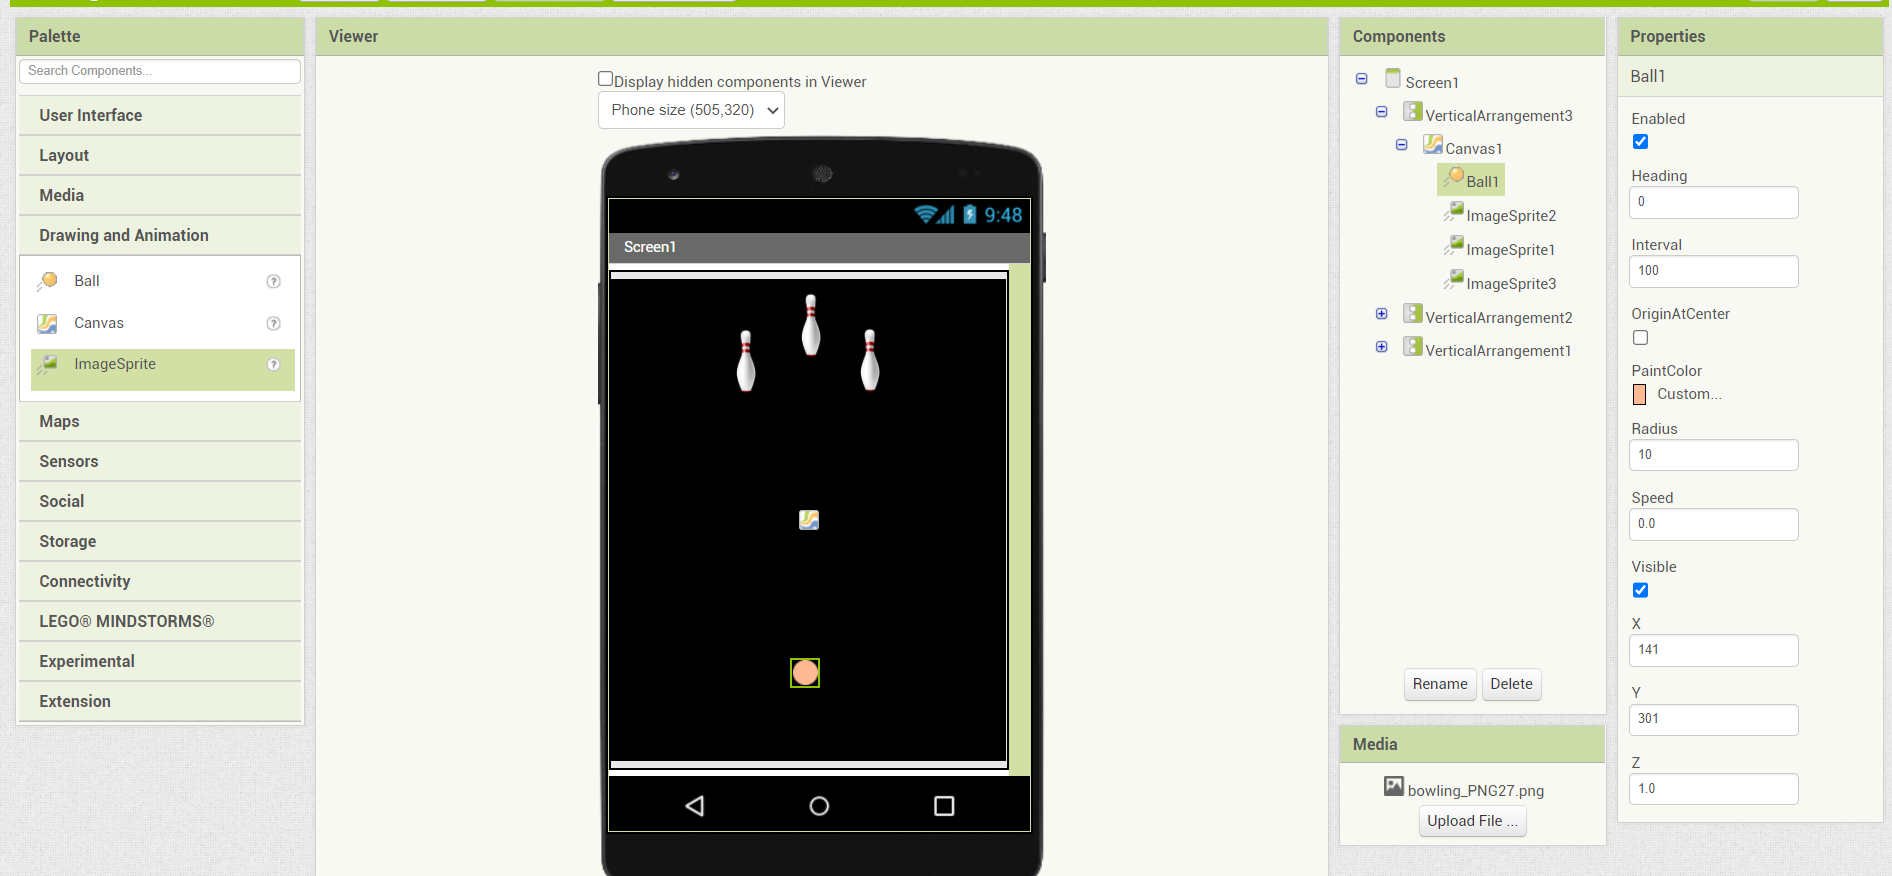
\includegraphics[width=1.0\linewidth,height=0.5\linewidth]{fig130009.png}
   \caption{Add the pins}
\label{fig130009}
\end{figure}

In the last part of the design, you should also add the ball launch button. First, add a HorizontalArrangement element. Change the width of the element to fit on the screen.

\begin{figure}[H]
   \centering
   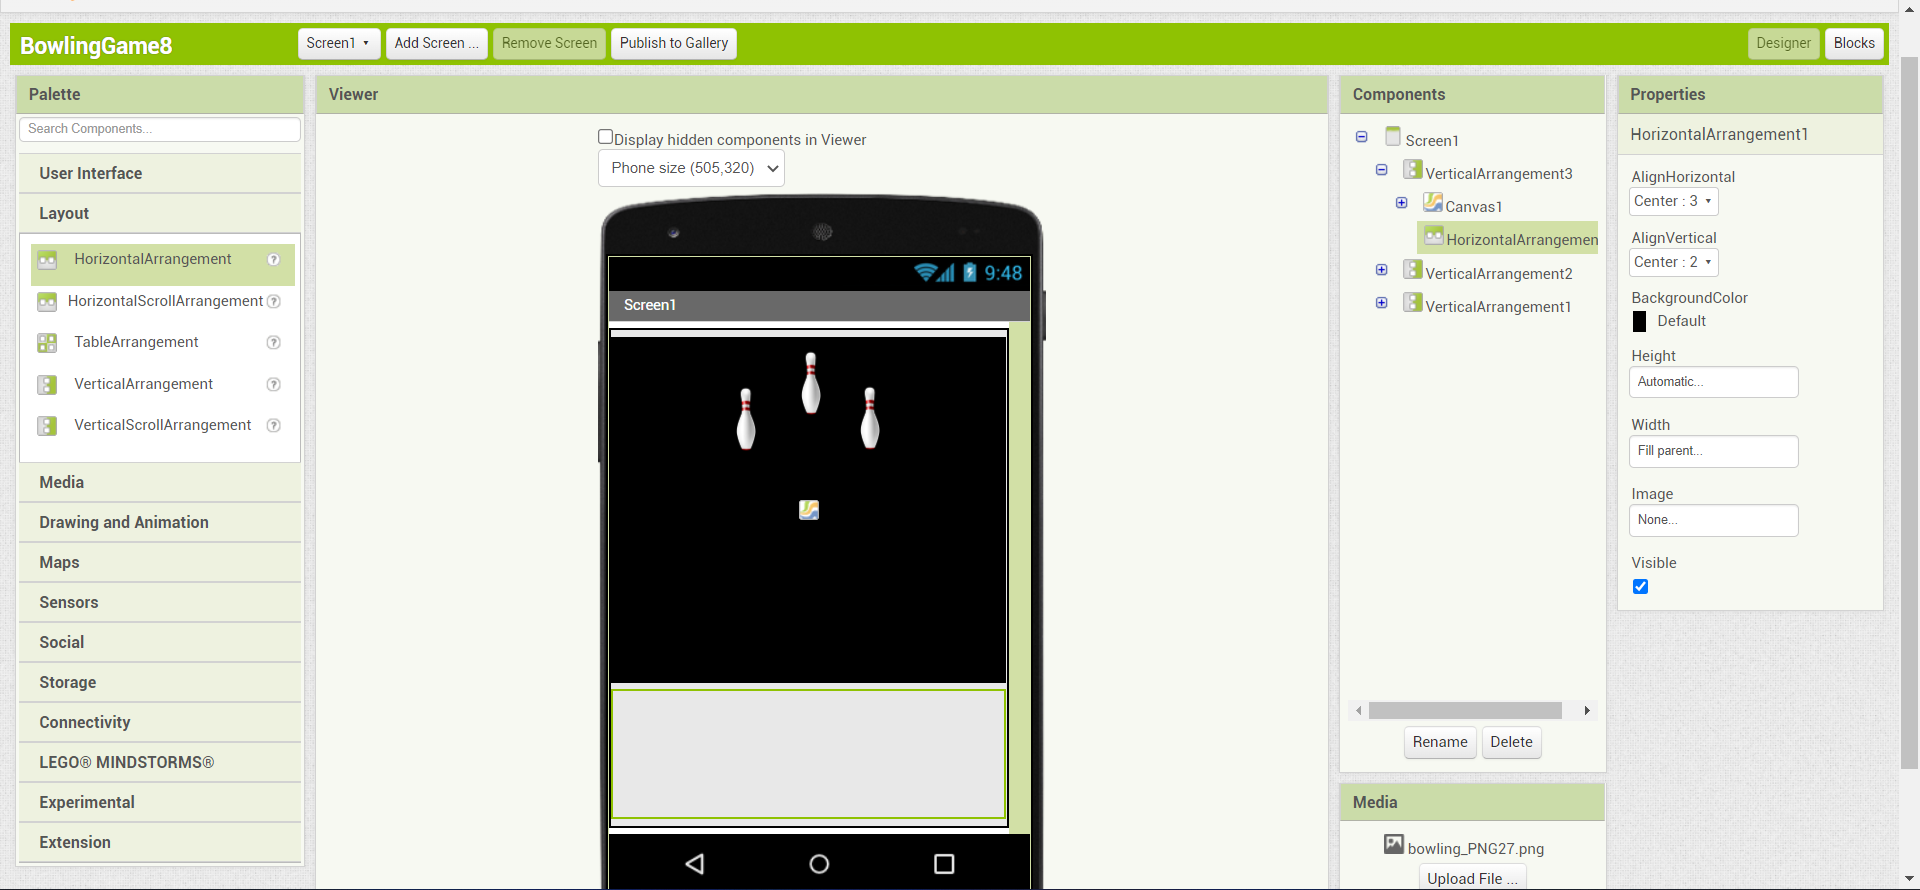
\includegraphics[width=1.0\linewidth,height=0.5\linewidth]{fig130010.png}
   \caption{Add space for shot button}
\label{fig130010}
\end{figure}

Add two more elements to this element - a button and an element that will display how many balls the character has. Position the elements and change the text of the elements. You can also change the color and shape.

\begin{figure}[H]
   \centering
   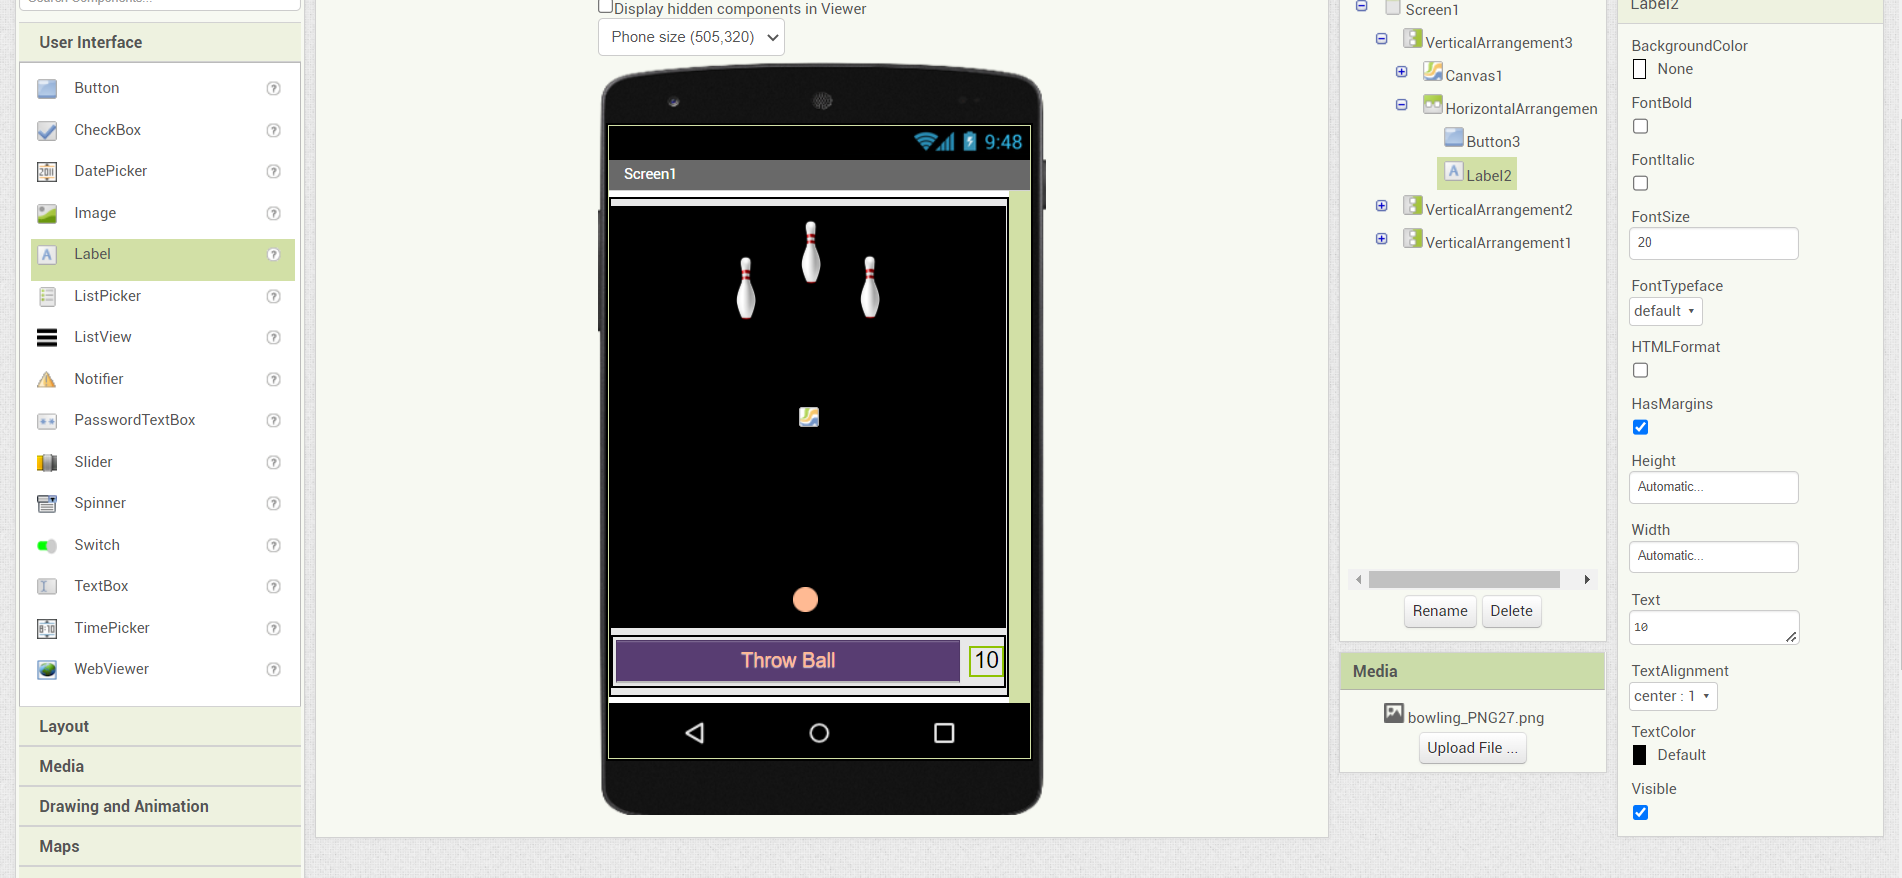
\includegraphics[width=1.0\linewidth,height=0.5\linewidth]{fig130011.png}
   \caption{Add button to shoot the ball}
\label{fig130011}
\end{figure}

\section{Creating the Program}

Before you start programming the game, leave only the game start screen visible. Then switch to the Add Blocks view.

Start by programming the game start button. Add the Click statement, which means that when the button is pressed, then the instructions will be executed. When this button is pressed it will set the speed of the ball.

\begin{figure}[H]
   \centering
   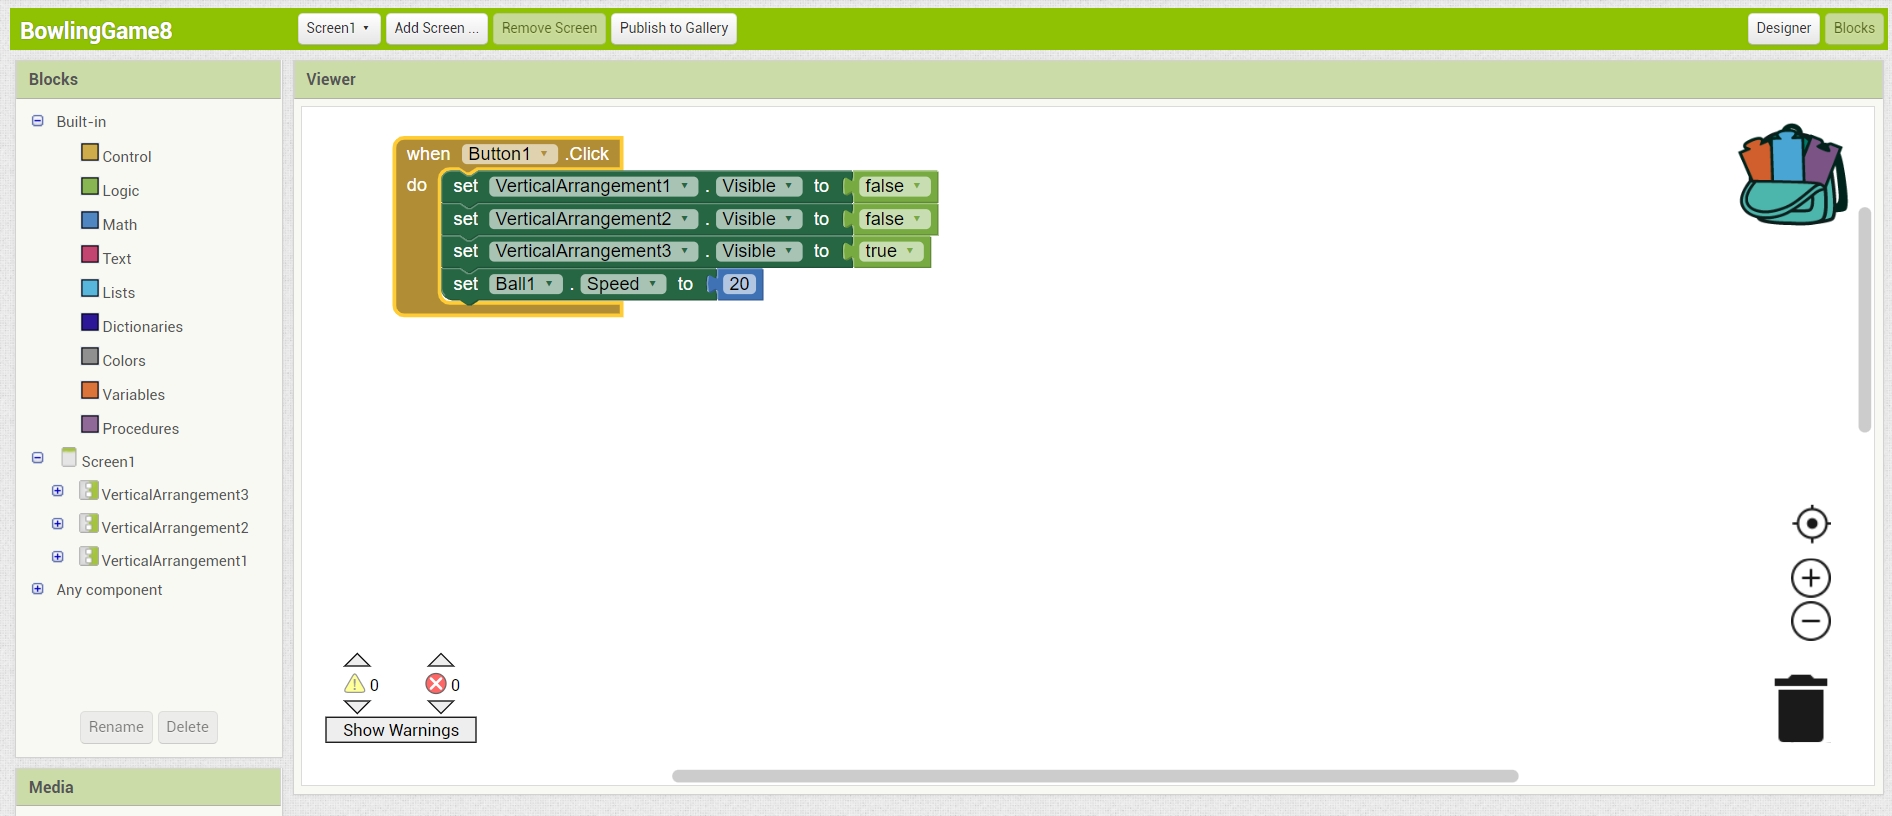
\includegraphics[width=1.0\linewidth,height=0.5\linewidth]{fig130012.png}
   \caption{Instructions for the home button}
\label{fig130012}
\end{figure}

Add a variable that will be the number of pins. Let the initial value be 3.

\begin{figure}[H]
   \centering
   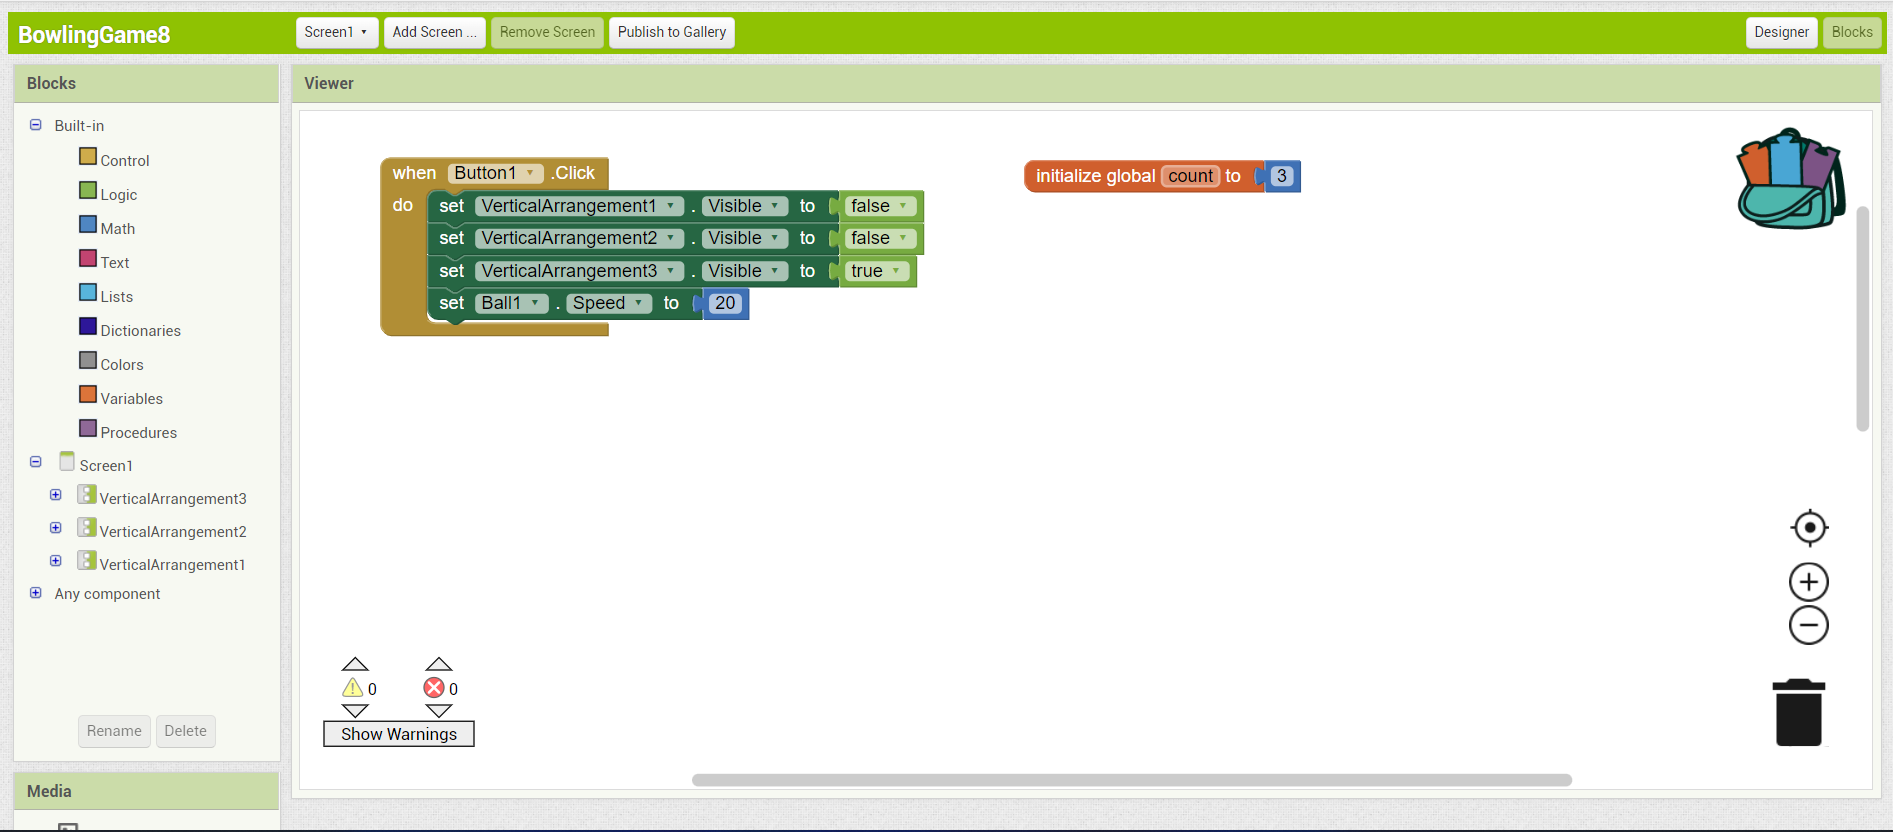
\includegraphics[width=1.0\linewidth,height=0.5\linewidth]{fig130013.png}
   \caption{Variable for the number of pins}
\label{fig130013}
\end{figure}

When the ball touches one of the edges it must deflect. To execute the ball deflection instructions, an event must first be added. Inside this event, the following checks must be done:
- if the ball is at the leftmost edge of the screen, it must move to the right
- if the ball is at the far right of the screen, it must move to the left
- if the ball is at the top edge of the screen, it must move to its original position.

\begin{figure}[H]
   \centering
   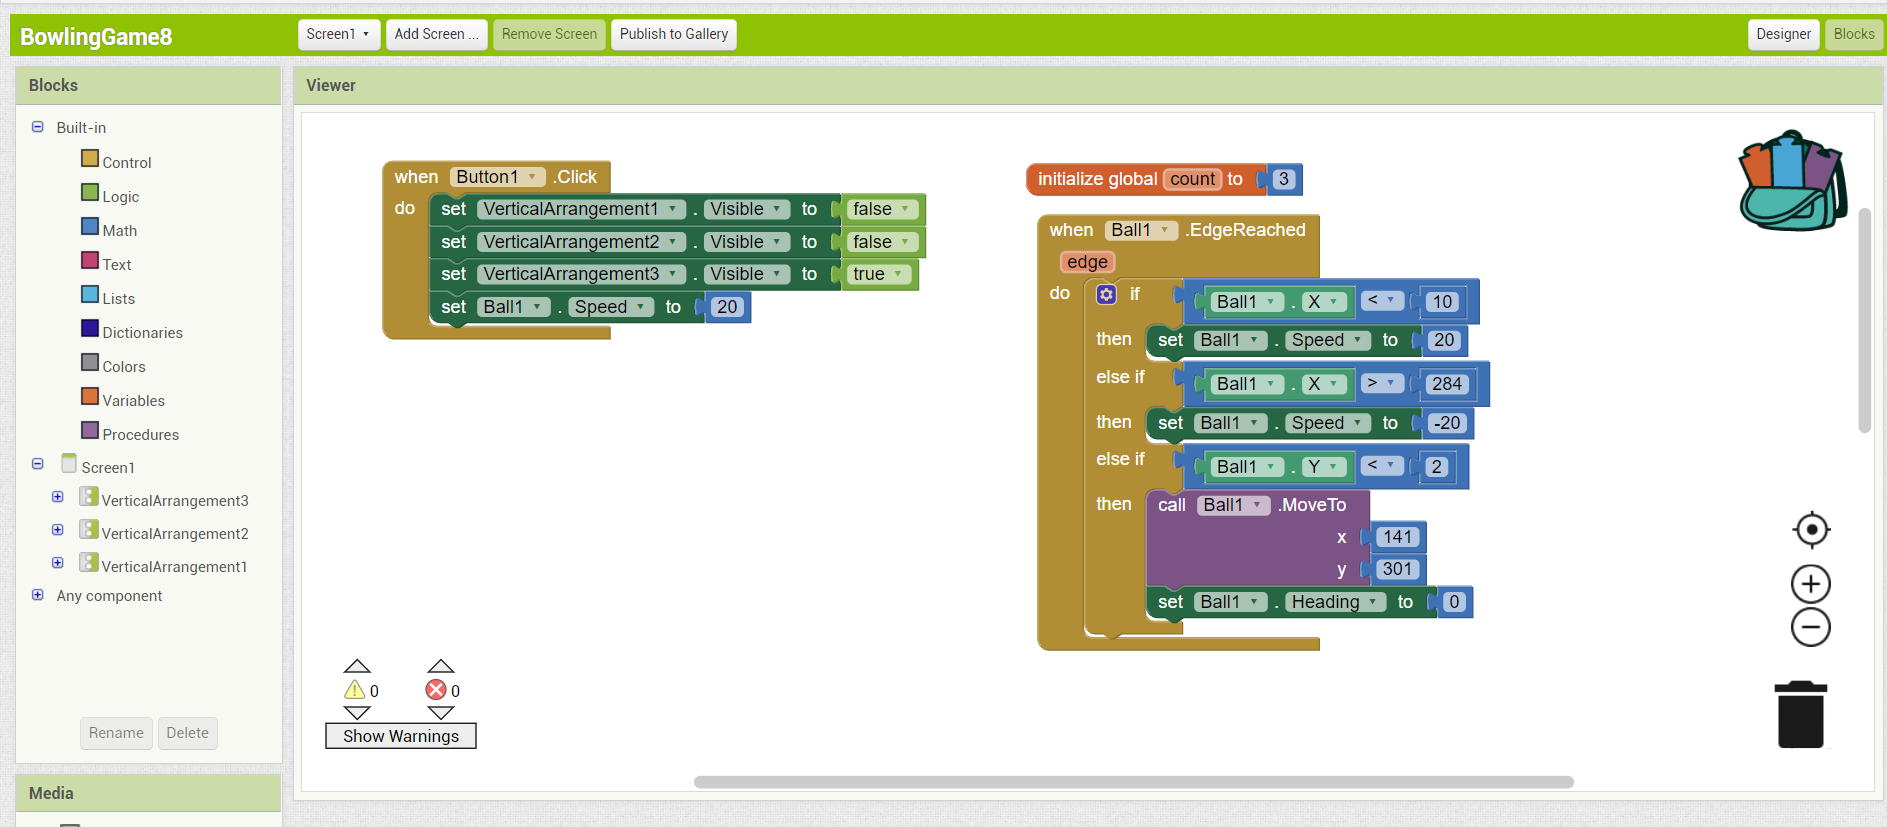
\includegraphics[width=1.0\linewidth,height=0.5\linewidth]{fig130014.png}
   \caption{Movement of the ball when it touches the edge of the screen}
\label{fig130014}
\end{figure}

The other event that applies to the ball is when it touches something other than the screen. In this game it can only be a pin. Then the number of pins must be changed by removing one. Another important thing to do is to check if there are more pins on the screen. If not, then this screen should be hidden and the last screen should be shown. It is important to change the message to say Winner.

If the number of pins is not equal to 0, then a check for which pin touched the ball must be added. The purpose of this is to be able to make it invisible and not be part of the game.

\begin{figure}[H]
   \centering
   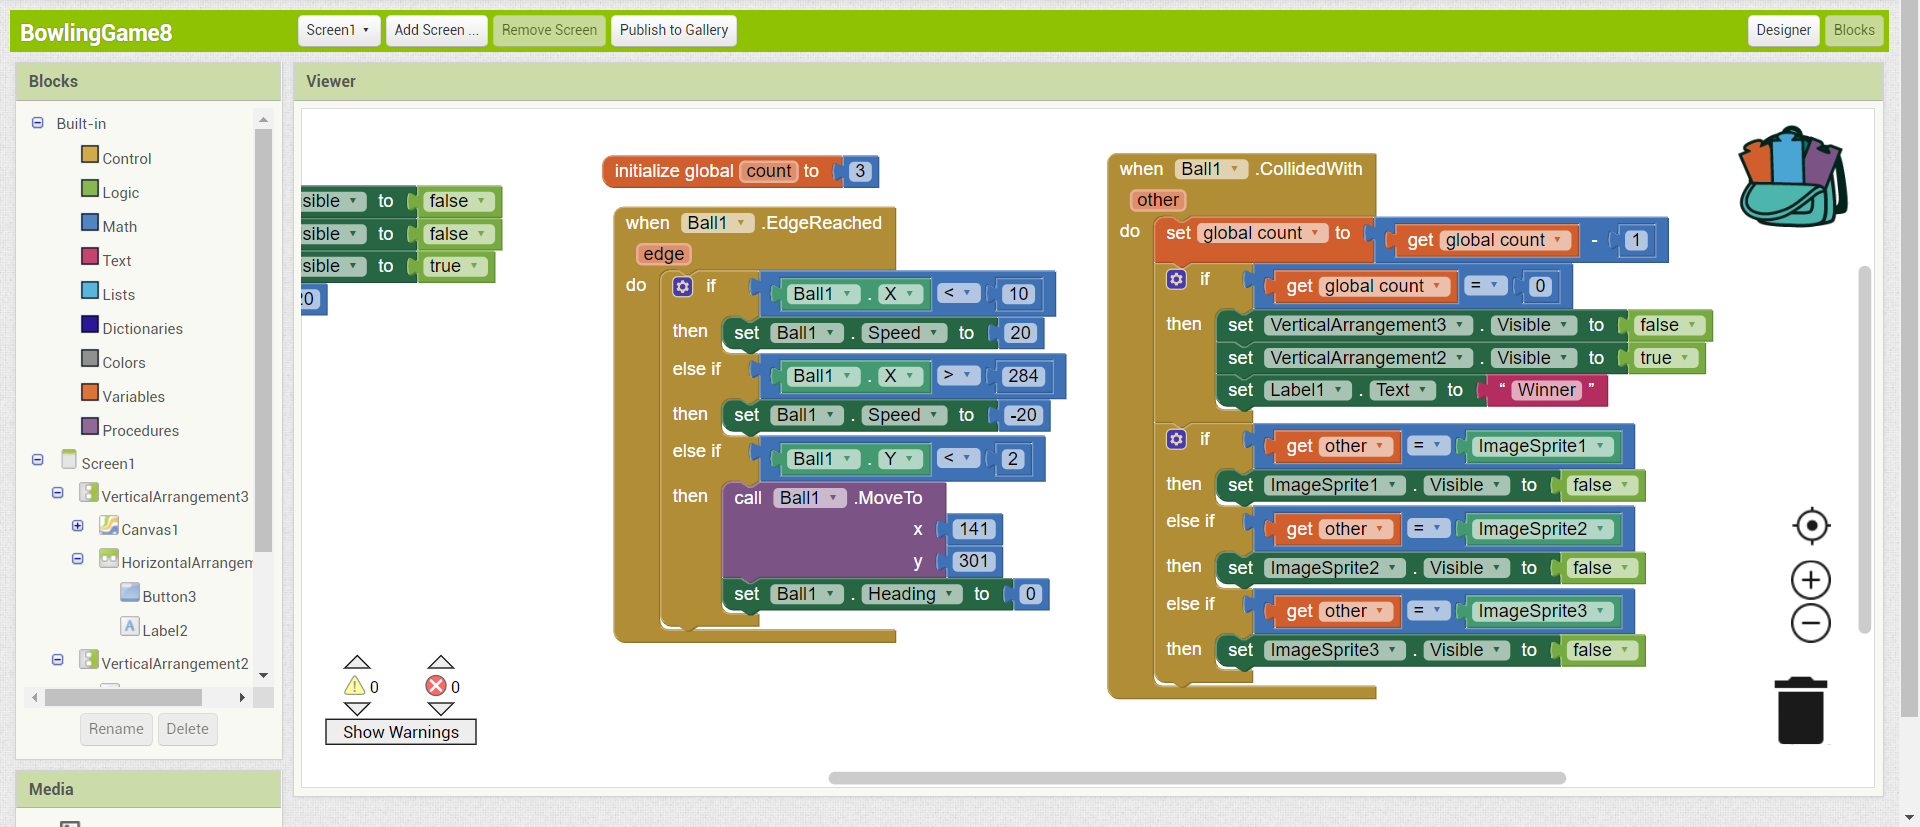
\includegraphics[width=1.0\linewidth,height=0.5\linewidth]{fig130015.png}
   \caption{Instructions when the ball hits the pin}
\label{fig130015}
\end{figure}

The next instructions will be when the ball launch button is pressed. The first check to be made is if the number of balls fired field is 0 then the game is over and the end of game screen should be displayed. If it is not equal to 0, then the direction of the ball should be set and the count should be decremented by 1.

\begin{figure}[H]
   \centering
   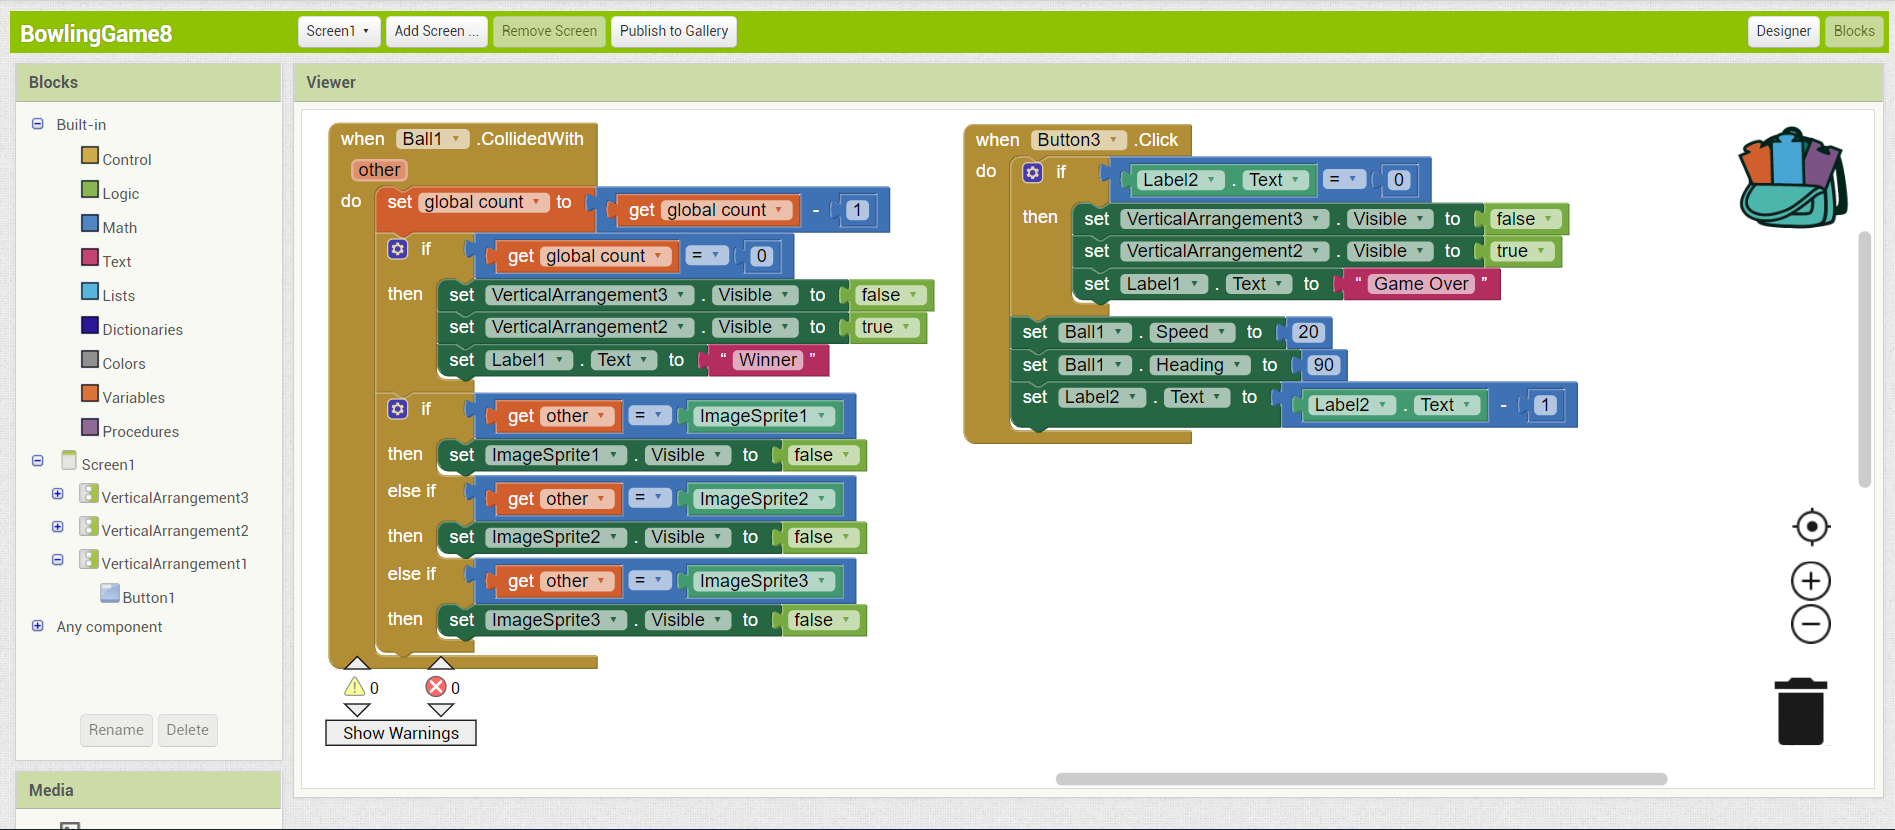
\includegraphics[width=1.0\linewidth,height=0.5\linewidth]{fig130016.png}
   \caption{Ball Shoot Button Instructions}
\label{fig130016}
\end{figure}

The last instructions to add are for the button that starts the game from the beginning. These instructions include displaying the game screen, displaying the pins, setting the number of pins to 3 and the number of balls to 10.

\begin{figure}[H]
   \centering
   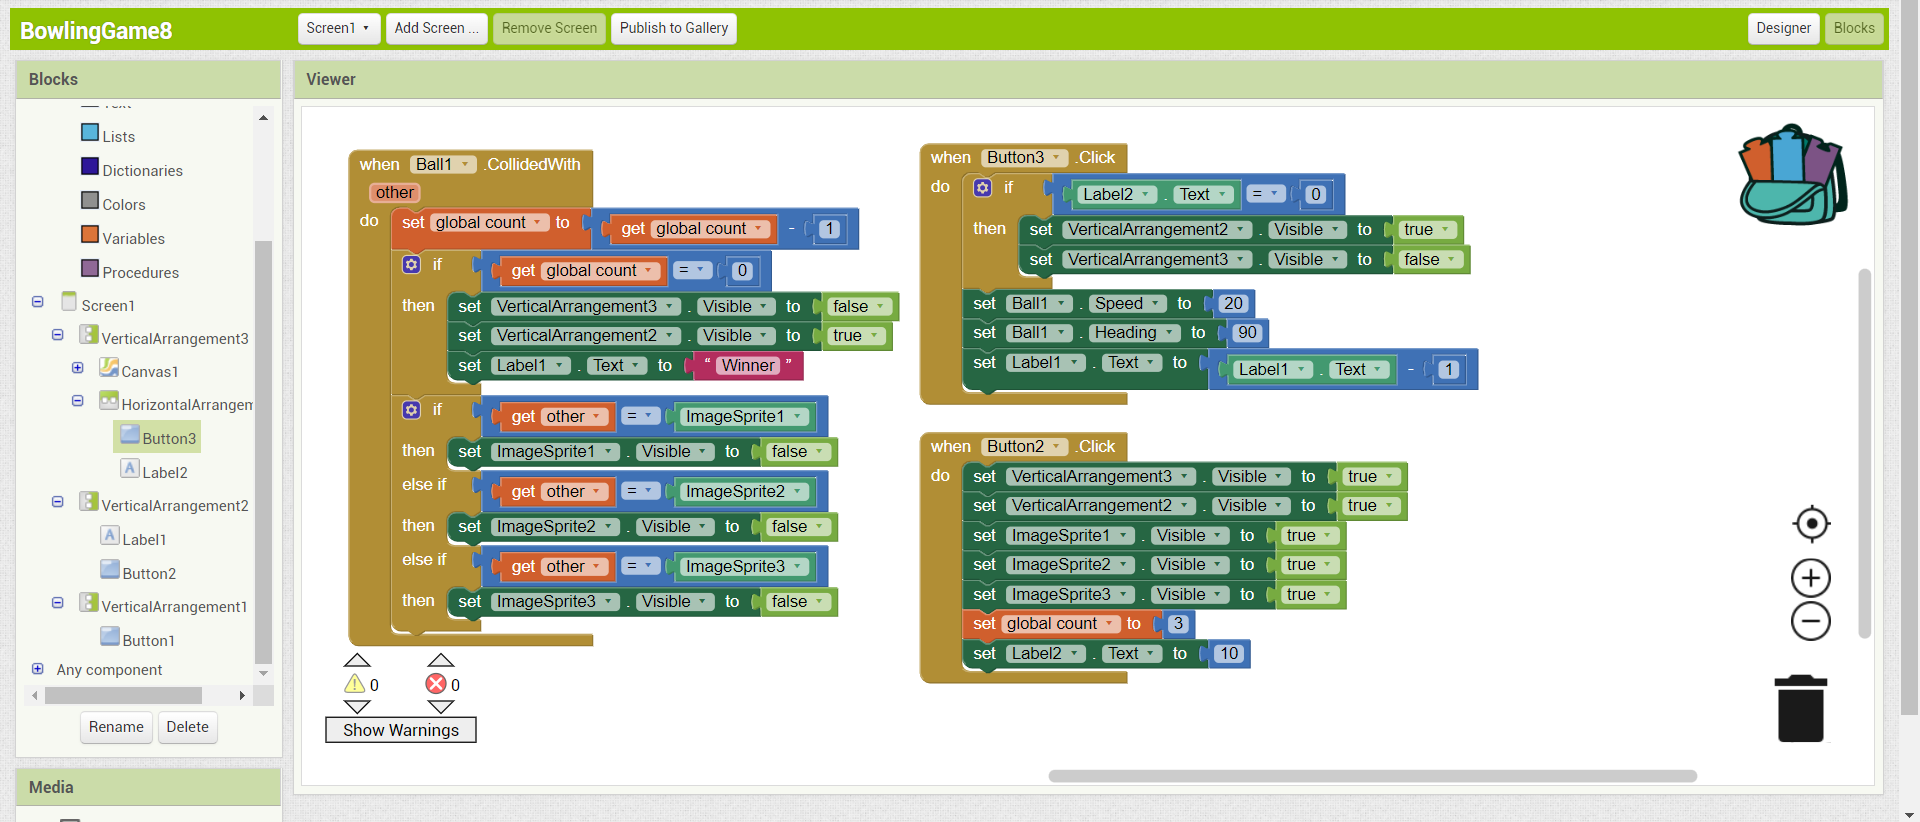
\includegraphics[width=1.0\linewidth,height=0.5\linewidth]{fig130017.png}
   \caption{Instructions for restart button}
\label{fig130017}
\end{figure}

We wish you a pleasant game!
